\documentclass[11pt]{article}

\usepackage[backend=bibtex,natbib,style=numeric-comp,sorting=none,doi=false,isbn=false,url=false]{biblatex}
\addbibresource{refs}

\usepackage[T1]{fontenc}
\usepackage{lmodern}
\usepackage{amsmath,amssymb,array,booktabs}
\usepackage{hyperref}
\usepackage[margin=1in]{geometry}
\usepackage{tikz}
\usetikzlibrary{arrows.meta,positioning}

\newcommand{\Aeff}{\alpha'_{\mathrm{eff}}}
\newcommand{\Sym}{\mathrm{Sym}}
\newcommand{\mc}[1]{\mathcal{#1}}
\newcommand{\bR}{\mathbb{R}}
\newcommand{\PLog}{\mathrm{PLog}}

\title{Chemical Potential, Winding, and the Orbifold/SYM Dictionary for the First-Order String}
\author{}
\date{}

\begin{document}
\maketitle

\section{Aim}
This note isolates one question in the curved first-order string proposal for the exact symmetric-orbifold CFT
\begin{equation}\label{eq:aim-orbifold}
\Sym^N(\bR^8).
\end{equation}
Why does the flat-torus genus-one comparison use a chemical potential, even though the exact orbifold CFT at fixed copy number $N$ is canonically defined? The short answer is that the chemical potential is not an extra local coupling of the orbifold CFT. It is the grand-canonical rewriting of the linear wound-string energy already present in the flat-torus Gomis--Ooguri benchmark \cite{gomis2000nonrelativisticclosedstringtheory}. This note also explains how that statement fits, and does not fit, with the NCOS/2d SYM flux-sector dictionary \cite{seiberg2000stringsbackgroundelectricfield,klebanov200011dimensionalncosun,gopakumar2000sdualitynoncommutativegaugetheory}.

The scope is deliberately narrow. I focus on the exact orbifold point and on the closed first-order string without a boundary. Comments about NCOS and full two-dimensional $\mathcal N=(8,8)$ $U(N)$ SYM are included only to clarify what is established, what is a flat-torus benchmark, and what is still open.

\section{Conventions and Scope}
The same letters are used in several nearby subjects, so I fix the conventions at the start:
\begin{equation}\label{eq:main-conventions}
N=\text{orbifold copy number and, in the SYM channel, gauge rank},
\end{equation}
\begin{equation}\label{eq:w-convention}
w=\text{cycle length of one twisted sector, equivalently one closed-string winding number},
\end{equation}
\begin{equation}\label{eq:k-convention}
k=\text{discrete electric-flux sector label of 2d }U(N)\text{ SYM}.
\end{equation}
Thus $N$, $w$, and $k$ are distinct quantities. In particular, the chemical potential discussed below couples to $w$ or to the total copy number in a generating function. It does not directly couple to the SYM flux label $k$.

I will also use the following standard parameters:
\begin{equation}\label{eq:parameter-conventions}
\begin{aligned}
\beta&=T^{-1},
\\
R&=\text{target-space spatial radius},
\\
\Aeff&=\text{effective string scale inherited from the NRCS limit}.
\end{aligned}
\end{equation}
For the flat thermal torus I write
\begin{equation}\label{eq:fugacity-convention}
p=e^{-\beta\mu},
\qquad
\mu=\frac{R}{2\Aeff},
\end{equation}
but the second equation is valid only in the flat-torus genus-one benchmark where the linear wound-string energy takes the simple form reviewed below.

There are three different layers in the discussion.
\begin{itemize}
\item The Poisson/BF core of the closed first-order string is the candidate exact dual of the orbifold data on the same two-dimensional spacetime $C$.
\item The finite $1/\Aeff$ term is a benchmark deformation imported from the Gomis--Ooguri thermal torus computation \cite{gomis2000nonrelativisticclosedstringtheory}. In that one-loop setting it supplies the linear winding energy and therefore the fugacity $p^w$.
\item The open-string NCOS theory on a D1-brane, and its dual description in a fixed SYM electric-flux sector, is a different system because it includes a boundary condition and a sector label $k$.
\end{itemize}
Whenever I import a formula from continuum non-relativistic string theory or from the standard symmetric-orbifold long-string literature, I say so explicitly.

\section{What the Chemical Potential Is on the String Side}
The cleanest starting point is the flat thermal torus benchmark imported from Gomis and Ooguri \cite{gomis2000nonrelativisticclosedstringtheory}. Their first-order worldsheet action contains a Poisson/BF term together with a finite $1/\Aeff$ deformation. In a sector with spatial winding number $w>0$, the zero-mode relation between the canonical target-space energy-momentum $(p_0,p_1)$ and the first-order zero modes is
\begin{equation}\label{eq:zero-mode-energy-momentum}
\frac{1}{2}(p_0+p_1)=i\beta_0+\frac{wR}{4\Aeff},
\qquad
\frac{1}{2}(p_0-p_1)=i\bar\beta_0+\frac{wR}{4\Aeff}.
\end{equation}
Here $\beta_0$ and $\bar\beta_0$ are the longitudinal first-order zero modes. The physical-state conditions then give
\begin{equation}\label{eq:beta0-weights}
i\beta_0=\frac{h}{wR},
\qquad
i\bar\beta_0=\frac{\bar h}{wR},
\end{equation}
where $h$ and $\bar h$ are the left- and right-moving transverse weights, including the transverse momentum contribution and oscillator contribution. Combining \eqref{eq:zero-mode-energy-momentum} and \eqref{eq:beta0-weights} gives the single-string energy
\begin{equation}\label{eq:single-string-energy}
E(w,h,\bar h)=p_0=\frac{wR}{2\Aeff}+\frac{h+\bar h}{wR}.
\end{equation}
Equation \eqref{eq:single-string-energy} is the key physics. The term linear in $w$ is not a new ensemble choice. It is part of the closed-string spectrum itself. It is the finite rest-energy cost per unit winding that survives the near-critical background-field subtraction in the non-relativistic closed-string limit.

The genus-one thermal free energy imported from \cite{gomis2000nonrelativisticclosedstringtheory} can then be written as
\begin{equation}\label{eq:go-free-energy-note}
F_{\mathrm{GO}}(T)=
T\sum_{w=1}^{\infty}
\sum_{\substack{h,\bar h\\ h-\bar h\in w\mathbb Z}}
D_w^{\mathrm{GO}}(h,\bar h)
\log\!\left(
1-e^{-\beta E(w,h,\bar h)}
\right),
\end{equation}
with $\beta=T^{-1}$. In the same one-loop computation, the worldsheet torus modulus localizes on holomorphic maps to the target thermal torus, and the longitudinal nonzero modes cancel against their fermionic partners. Because of that special cancellation, the finite $1/\Aeff$ term contributes only the instanton factor
\begin{equation}\label{eq:instantonic-boltzmann}
e^{-\beta wR/(2\Aeff)}.
\end{equation}
At this stage one simply rewrites that Boltzmann factor as
\begin{equation}\label{eq:chemical-potential-rewrite}
e^{-\beta wR/(2\Aeff)}=p^w,
\qquad
p=e^{-\beta\mu},
\qquad
\mu=\frac{R}{2\Aeff}.
\end{equation}
This is why the term ``chemical potential'' appears. It is a convenient thermodynamic name for a quantity that, from the string point of view, is already the rest-energy per unit winding. The worldsheet theory does not gain a new local coupling when one writes \eqref{eq:chemical-potential-rewrite}; one has only repackaged the linear piece of \eqref{eq:single-string-energy}.

So the correct string-side interpretation is:
\begin{itemize}
\item \emph{before} rewriting the partition function, $\mu$ is just the coefficient of the linear winding energy in the spectrum;
\item \emph{after} rewriting the partition function in second-quantized form, the same coefficient becomes the fugacity conjugate to total winding or total copy number.
\end{itemize}
The word ``chemical potential'' belongs to the second description, not to the local worldsheet dynamics.

\section{Canonical Orbifold Data Versus Grand-Canonical Packaging}
The exact symmetric product $\Sym^N(\bR^8)$ is canonically defined at fixed $N$. If $Z_N^{\Sym}(\beta)$ denotes its thermal partition function on the target thermal circle of circumference $\beta$, then one may package the whole family $\{Z_N^{\Sym}\}_{N\ge 0}$ into the generating function
\begin{equation}\label{eq:orbifold-generating-function}
\mc Z_{\Sym}(\beta,p)=\sum_{N=0}^{\infty} p^N Z_N^{\Sym}(\beta).
\end{equation}
The canonical answer at fixed $N$ is recovered by coefficient extraction,
\begin{equation}\label{eq:coefficient-extraction}
Z_N^{\Sym}(\beta)=[p^N]\mc Z_{\Sym}(\beta,p).
\end{equation}
Thus the fugacity $p$ is optional bookkeeping. It is not part of the definition of one fixed orbifold theory.

For the order-$N^0$ single-cycle contribution relevant to the genus-one benchmark, the standard Dijkgraaf--Verlinde--Verlinde long-string description \cite{dijkgraaf1997matrixstring,dijkgraaf1997ellipticgenerasymmetricproducts,arutyunov1998orbifoldscattering} gives
\begin{equation}\label{eq:orbifold-free-energy-note}
F_{\Sym}^{(0)}(\beta,p)\Big|_{[1,0]}
=
T\sum_{w=1}^{\infty}
\sum_{\substack{h,\bar h\\ h-\bar h\in w\mathbb Z}}
D_{\rm RR}^{\mathrm{seed}}(h,\bar h)
\log\!\left(
1-p^w e^{-\beta(h+\bar h)/(wR)}
\right).
\end{equation}
Here $D_{\rm RR}^{\mathrm{seed}}(h,\bar h)$ is the degeneracy of one copy of the free $(8,8)$ seed theory on $\bR^8$ in the physical thermal spin structure with periodic spatial fermions. Equation \eqref{eq:orbifold-free-energy-note} is still built from exact orbifold data. The only grand-canonical ingredient is the external packaging variable $p$.

Comparing \eqref{eq:orbifold-free-energy-note} with the string formula \eqref{eq:go-free-energy-note} shows that the two agree term by term once one identifies
\begin{equation}\label{eq:benchmark-match}
p=e^{-\beta R/(2\Aeff)}.
\end{equation}
This is the precise meaning of the flat-torus match. The finite $1/\Aeff$ deformation does not change the intrinsic local dynamics of $\Sym^N(\bR^8)$ at fixed $N$. It only tells us which generating function of canonical orbifold data reproduces the thermal one-loop string answer.

The same distinction is even clearer for local observables. For example, a connected three-point function of normalized single-cycle twist operators,
\begin{equation}\label{eq:canonical-three-point}
\mc C_{123}^{(g)}(N)=
\bigl\langle
\widehat{\sigma}_{[w_1]}(0)\,
\widehat{\sigma}_{[w_2]}(1)\,
\widehat{\sigma}_{[w_3]}(\infty)
\bigr\rangle_{g}^{\mathrm{conn}},
\end{equation}
is a canonical fixed-$N$ orbifold observable. It does not structurally require any fugacity. On the first-order-string side, the natural classical saddles are branched covers with local ramification indices $(w_1,w_2,w_3)$, but the full BRST-complete measure on that branched-cover locus is still open \cite{lunin2001correlationorbifolds,lunin2002threepointorbifolds,pakman2009diagramssymmetricorbifold,pakman2009extremalhurwitz}.

\section{Dictionary and Status}
Table \ref{tab:dictionary} separates what is established from what is only a flat-torus benchmark or still open.

\begin{table}[ht]
\centering
\renewcommand{\arraystretch}{1.2}
\begin{tabular}{>{\raggedright\arraybackslash}p{0.21\linewidth} >{\raggedright\arraybackslash}p{0.52\linewidth} >{\raggedright\arraybackslash}p{0.20\linewidth}}
\toprule
Worldsheet quantity & Orbifold or SYM meaning & Status \\
\midrule
$w$ & One closed-string winding number on the target spatial circle; one cycle length in the symmetric product & Exact in the flat-torus benchmark \\
$n$-sum modulo $w$ & $\mathbb Z_w$ projector onto states invariant under the cyclic permutation in the length-$w$ twisted sector & Exact in the flat-torus benchmark \\
$m$-sum & Plethystic expansion of the single-cycle contribution, equivalently the standard $\log(1-x)$ second-quantized free-gas factor & Exact in the flat-torus benchmark \\
$D_w(h,\bar h)$ & Seed-state multiplicity. In the physical thermal spin structure and standard DVV lift it reduces to $D_{\rm RR}^{\mathrm{seed}}(h,\bar h)$ & Exact in the flat-torus benchmark \\
$p=e^{-\beta\mu}$ & Fugacity conjugate to total copy number in the generating function, with $\mu$ rewritten from the linear winding energy & Bookkeeping for the benchmark \\
finite $1/\Aeff$ term & Supplies the linear winding energy $wR/(2\Aeff)$ in the genus-one thermal benchmark & Benchmark for the orbifold match \\
fixed-$N$ twist correlators & Canonical observables of the exact orbifold CFT, for example \eqref{eq:canonical-three-point} & Exact on the orbifold side; string realization still open \\
branched-cover saddles on $S^2$ & Classical first-order-string localization locus for twist insertions of given cycle lengths & Classical locus clear; quantum measure still open \\
$k$ in 2d SYM & Electric-flux superselection sector of $U(N)$ SYM; relevant for NCOS with a boundary, not for the pure closed benchmark by itself & Separate NCOS/SYM input \\
\bottomrule
\end{tabular}
\caption{Status of the proposed dictionary. ``Exact'' here means exact within the specific observable and conventions stated nearby. The flat-torus genus-one benchmark is strong but does not yet determine the full curved-target or full-SYM completion.}
\label{tab:dictionary}
\end{table}

Figure \ref{fig:bookkeeping-map} summarizes the logical relations among the four nearby theories. The important point is that the flat-torus chemical potential belongs on the benchmark arrow, not on the fixed-$N$ orbifold node and not on the full-SYM node.

\begin{figure}[ht]
\centering
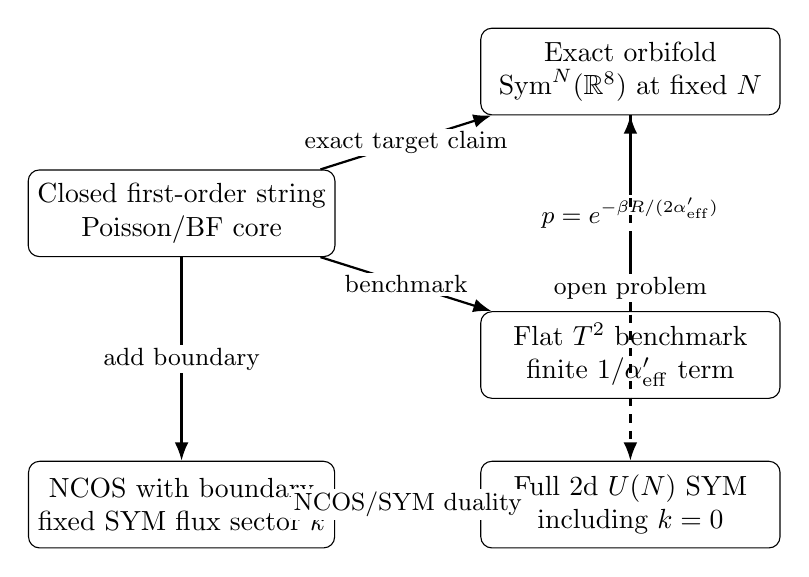
\begin{tikzpicture}[
  box/.style={draw, rounded corners, align=center, minimum width=3.8cm, minimum height=1.1cm},
  lab/.style={midway, fill=white, inner sep=1pt, font=\small},
  >=Latex
]
\node[box] (core) at (0,0) {Closed first-order string\\Poisson/BF core};
\node[box] (orb) at (5.7,1.8) {Exact orbifold\\$\Sym^N(\bR^8)$ at fixed $N$};
\node[box] (bench) at (5.7,-1.8) {Flat $T^2$ benchmark\\finite $1/\Aeff$ term};
\node[box] (ncos) at (0,-3.7) {NCOS with boundary\\fixed SYM flux sector $k$};
\node[box] (sym) at (5.7,-3.7) {Full 2d $U(N)$ SYM\\including $k=0$};

\draw[->, thick] (core) -- node[lab] {exact target claim} (orb);
\draw[->, thick] (core) -- node[lab] {benchmark} (bench);
\draw[->, thick] (bench) -- node[lab] {$p=e^{-\beta R/(2\Aeff)}$} (orb);
\draw[->, thick] (core) -- node[lab] {add boundary} (ncos);
\draw[->, thick, dashed] (ncos) -- node[lab] {NCOS/SYM duality} (sym);
\draw[->, thick, dashed] (orb) -- node[lab] {open problem} (sym);
\end{tikzpicture}
\caption{Bookkeeping map for the nearby theories. The mathematical role of the figure is to keep separate the exact fixed-$N$ orbifold, the flat-torus benchmark that introduces the fugacity $p$, the NCOS boundary sector tied to a fixed SYM flux label $k$, and the still-open extension to full SYM.}
\label{fig:bookkeeping-map}
\end{figure}

\section{Relation to NCOS and Full SYM}
The NCOS/SYM dictionary adds one ingredient that is absent from the pure closed first-order benchmark: a D1-brane boundary condition. In the open-string theory on that D1-brane, the dual gauge theory is 2d $\mathcal N=(8,8)$ $U(N)$ SYM in a fixed electric-flux superselection sector labeled by $k\in \mathbb Z_N$ \cite{seiberg2000stringsbackgroundelectricfield,klebanov200011dimensionalncosun,gopakumar2000sdualitynoncommutativegaugetheory,yin2026foundationsofstringtheory,cho2026fluxsectorsmatrixstring}. The ground-state energy density in that sector is
\begin{equation}\label{eq:sym-flux-energy-note}
E_k=\frac{k^2 g_{\rm YM}^2}{2N},
\end{equation}
and the corresponding diagonal electric flux density is
\begin{equation}\label{eq:sym-flux-density-note}
F_{01}^{\rm diag}=\frac{k g_{\rm YM}^2}{N}.
\end{equation}
So the near-critical electric field of the NCOS description is fixed by the flux sector and the couplings. It is not an independent continuous control parameter.

This is conceptually different from the flat-torus fugacity $p$. The closed-string chemical potential discussed above is conjugate to total winding,
\begin{equation}\label{eq:total-winding-weight-note}
\prod_a p^{w_a}=e^{-\beta\mu\sum_a w_a},
\end{equation}
where the sum runs over the cycles present in a multi-string or multi-cycle state. In the orbifold generating function the same weight is conjugate to total copy number. By contrast, the SYM label $k$ specifies a superselection sector of the gauge theory. Therefore:
\begin{itemize}
\item $w$ organizes one long string or one orbifold cycle;
\item $N$ fixes the total orbifold copy number and the SYM rank;
\item $k$ selects the SYM electric-flux sector relevant to NCOS with a boundary.
\end{itemize}
The chemical potential of the closed flat-torus benchmark should therefore not be identified with the SYM flux label.

This also explains why one does \emph{not} reach zero-flux SYM by simply setting $\mu=0$. Setting $\mu=0$ removes the linear winding term from the particular grand-canonical benchmark \eqref{eq:orbifold-free-energy-note}. It does not produce the full canonical $k=0$ gauge theory, and it does not explain how the pure closed first-order string should reorganize the complete SYM Hilbert space. Reaching full SYM, especially the $k=0$ sector, would require an additional ingredient not yet derived. Logical possibilities include:
\begin{itemize}
\item a deformation of the closed Poisson/BF worldsheet theory away from the exact orbifold point;
\item a more complete sum over sectors that treats the boundary and bulk data together;
\item a different observable map in which the closed first-order string captures only a subsector of SYM and must be supplemented by extra data.
\end{itemize}
At present the available evidence does not choose uniquely among these options.

\section{Takeaway}
The comparison can be stated precisely.
\begin{itemize}
\item The chemical potential in the flat-torus Gomis--Ooguri/orbifold match is the grand-canonical rewriting of the linear winding energy $wR/(2\Aeff)$. From the string point of view it is rest energy first and fugacity second.
\item The exact symmetric-orbifold CFT is canonically defined at fixed $N$. Grand-canonical variables are useful because they package the family of canonical theories and make the genus-one second-quantized comparison transparent, but they do not deform the local orbifold dynamics.
\item The NCOS/SYM flux-sector story is related but distinct. The SYM flux label $k$ belongs to the open-string boundary problem. The pure closed first-order string benchmark does not yet yield the full two-dimensional SYM theory, and zero-flux SYM is not obtained by simply turning off the fugacity.
\end{itemize}

So the exact correspondence currently supported is the following. The Poisson/BF first-order string, together with the eight transverse free multiplets, reorganizes exact orbifold data in a string-theoretic way. At genus one on the flat thermal torus, the finite $1/\Aeff$ benchmark deformation adds the linear winding energy and therefore selects a natural generating function of those orbifold data. Beyond that benchmark, canonical fixed-$N$ observables such as twist-sector correlators remain the right target on the orbifold side, while the extension toward matrix string theory or full 2d SYM remains a separate open deformation problem.

\printbibliography

\end{document}
